\documentclass[12pt]{article}

\usepackage[hmargin=2.5cm, vmargin={3cm,3cm}, a4paper]{geometry} 
\usepackage{amsmath,amssymb,amsthm,mathrsfs}
\usepackage{epsfig,epsf,subfigure,graphicx,graphics}
\usepackage{float}
\usepackage{url,enumerate}
\usepackage{listings}
\usepackage{ragged2e}
\graphicspath{{fig/}}
\usepackage{fancyhdr}
\usepackage{hyperref}
\hypersetup{
    colorlinks=true,
    linkcolor=blue,
    filecolor=magenta,      
    urlcolor=cyan,
    pdfpagemode=FullScreen,
    }
\setlength{\headheight}{12pt}
\pagestyle{fancyplain}

\graphicspath{ {./images/} }%Path to the images
 
\rhead{}
\lhead{}
\chead{{\it Graph Signal Processing Course, ETSETB}}
\lfoot{}
\cfoot{\thepage}
\rfoot{}
\title{Graph Fourier Transform}
\author{Gerard Castell}
\begin{document}
\maketitle

\thispagestyle{fancyplain}
\flushleft 


\Large
\hspace{10pt}
\small
\section{Activity}
\justifying
The image selected for this experiment is the following:
\begin{figure}[H]
	\centering
	
\includegraphics[width=3cm]{thunder.png}
	\caption{Image of a thunder, 50x50px}
	\label{fig:graphRepresentation}
\end{figure}
%%First subsection
\subsection{Build a regular grid}
\justifying
First of all, I have processed the thunder image and build a graph from the binarized image, resulting in \href{fig:3DnormLapl3clusters}{next graph}. As we may observe, we have obtained an undirected connected graph and there are no isolated communities.
\begin{figure}[H]
	\centering
	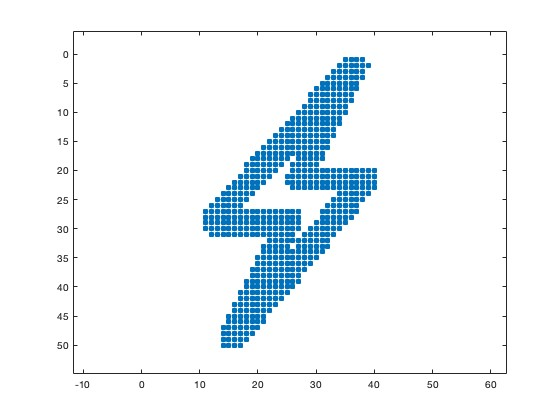
\includegraphics[width=12cm]{thunder_graph.jpg}
	\caption{Graph built from the initial image}
	\label{fig:GraphFromImage}
\end{figure}

\subsection{Spectral analysis of the undirected unweighted graph}
\justifying
In the Graph Fourier Transform the eigenvalues take the role of the frequencies and the eigenvectors the Fourier basis. In the image below, we may notice the relation between eigenvalues and spatial variation across the graph. We can observe from the second eigenvector how the graph starts to project where the variations are higher or lower depending on the edges weights.
\begin{figure}[H]
	\centering
	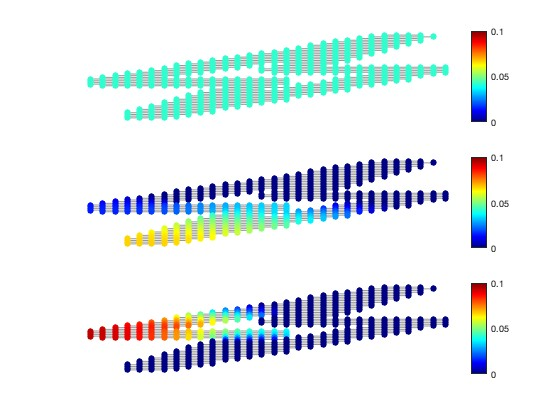
\includegraphics[width=12cm]{thunder_graph_2d_123ev.jpg}
	\caption{Spectral analysis of the graph for the first three eigenvectors}
	\label{fig:Graphd2dFirstEV}
\end{figure}
Now, we can plot the representation of graph signals in 3D. So the resulting image is the following for the second eigenvector:

\begin{figure}[H]
	\centering
	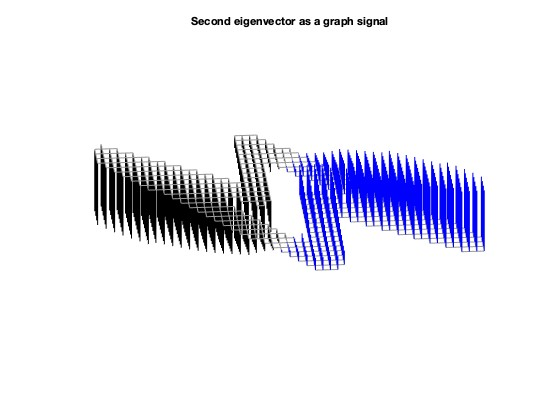
\includegraphics[width=12cm]{thunder_3d_123ev.jpg}
	\caption{Spectral analysis 3D-representation of the graph for the 1st, 2nd and 3rd eigenvectors}
	\label{fig:Graphd3dFirstEV}
\end{figure}
\subsection{Next eigenvectors as graph signals}
\justifying
Let's see what happens in the following eigenvectors.
\begin{figure}[H]
	\centering
	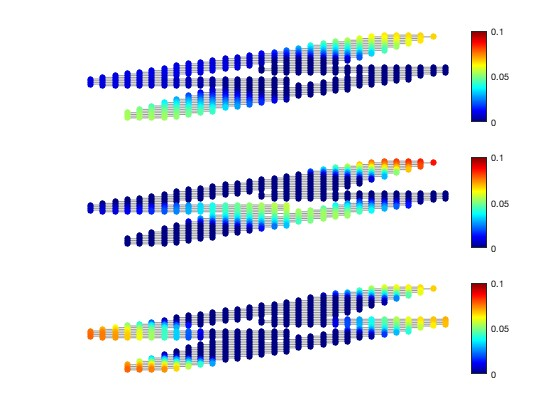
\includegraphics[width=12cm]{thunder_graph_2d_456ev.jpg}
	\caption{Spectral analysis of the graph for the 4th, 5th and 6th eigenvectors}
	\label{fig:Graphd2dSecondEV}
\end{figure}
\justifying
We can also plot the representation of graph signals in 3D for such eigenvectors. Hence, in the resulting image for the 6th eigenvector we may observe a variation in the edges of the thunder where the variation has been split up and localized in 4 parts:
\begin{figure}[H]
	\centering
	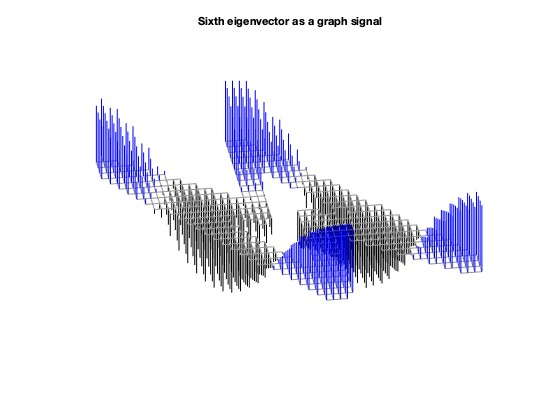
\includegraphics[width=12cm]{thunder_3d_456ev.jpg}
	\caption{Spectral analysis 3D-representation of the graph for the 4th, 5th and 6th eigenvectors}
	\label{fig:Graphd3dSecondEV}
\end{figure}

\subsection{Adding new edges}
To the initial graph we have added some new edges: [43 17; 31 14; 30 11; 45 15; 31 19; 28 16; 46 18]; 
The resulting graph with this modifications is the following:
\begin{figure}[H]
	\centering
	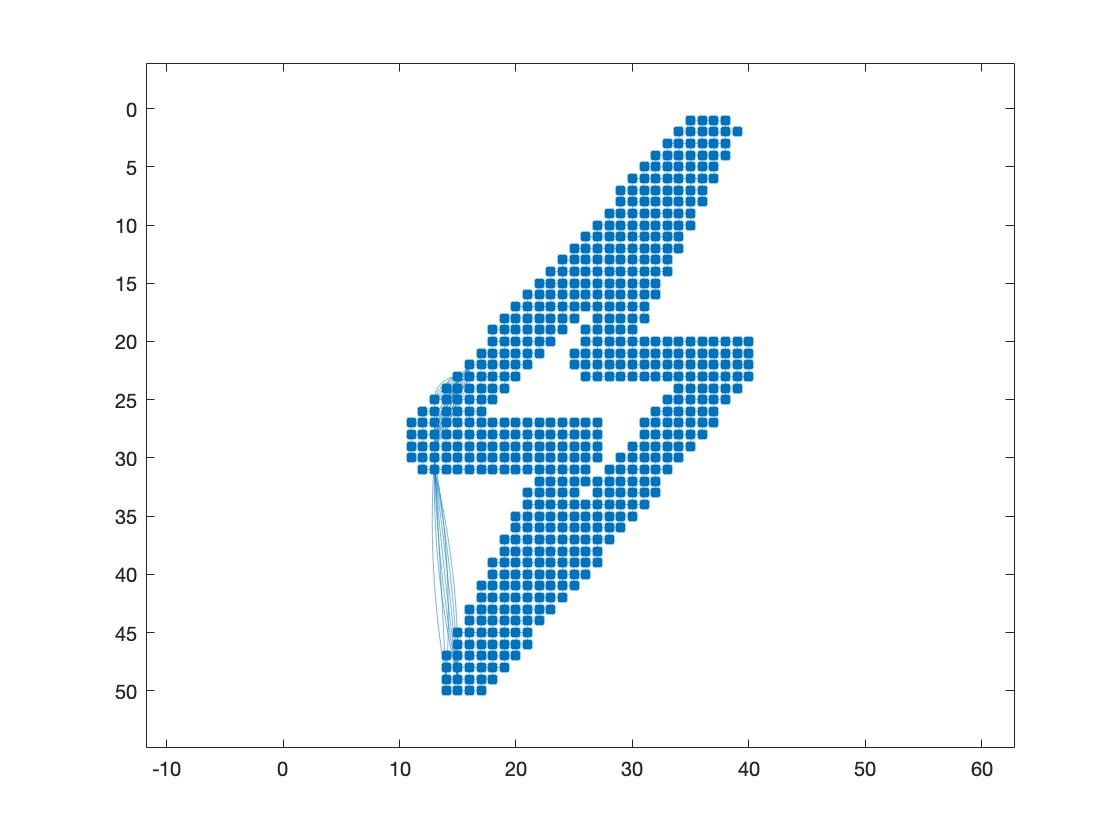
\includegraphics[width=12cm]{graph_more_edges.jpg}
	\caption{Initial graph with added edges}
	\label{fig:MoreEdgesGraph}
\end{figure}
With that variation, if we observe the Spectral representation we can observe the change across the graph, since the signal is going to be projected differently. Hence, we can appreciate such a behaviour in the image below:
\begin{figure}[H]
	\centering
	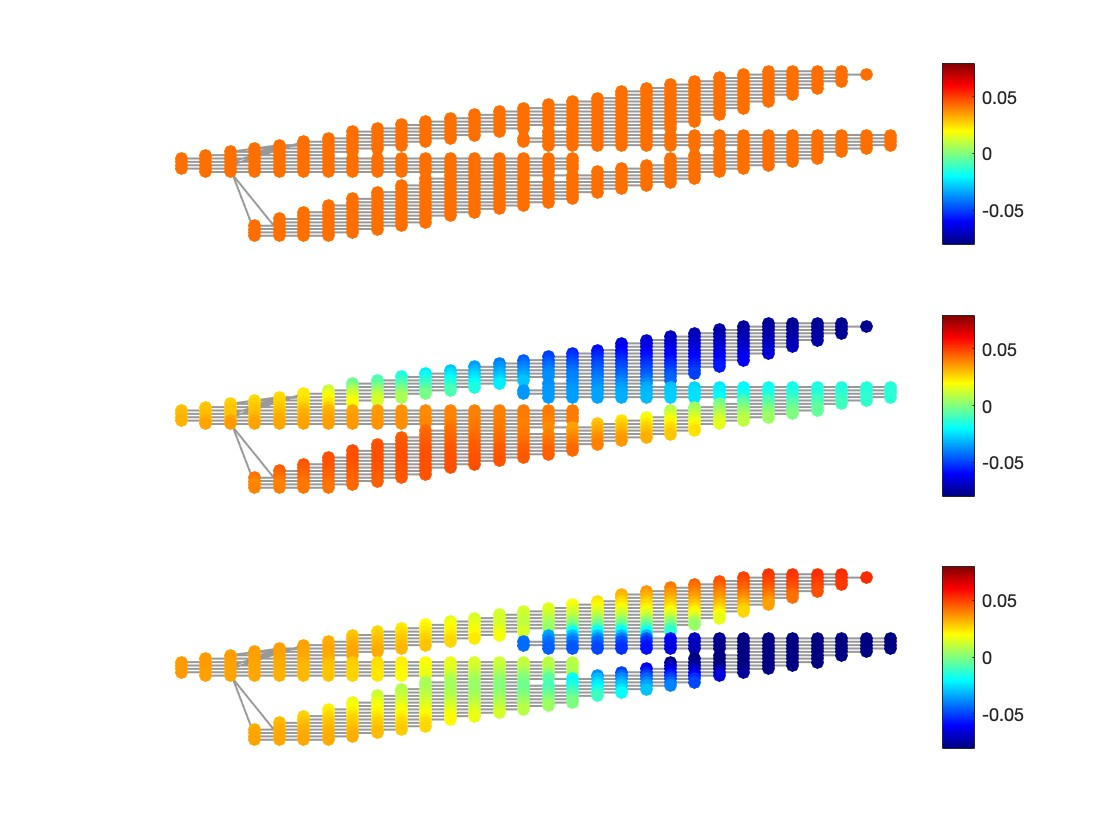
\includegraphics[width=12cm]{more_edges.jpg}
	\caption{Spectral analysis of the graph for the 1st, 2nd and 3rd eigenvectors with more edges}
	\label{fig:MoreEdgesSpectralRepresentation}
\end{figure}

If we focus on the following eigenvectors composition, we can see that the variation keeps propagating across the graph and the variation really changes the projection. In the initial graph we found a symmetric convergence in the graph on the edges of the thunder, however in the graph with more edges we notice that there more variation on the part where the new edges have been added, which makes totally sense.
\begin{figure}[H]
	\centering
	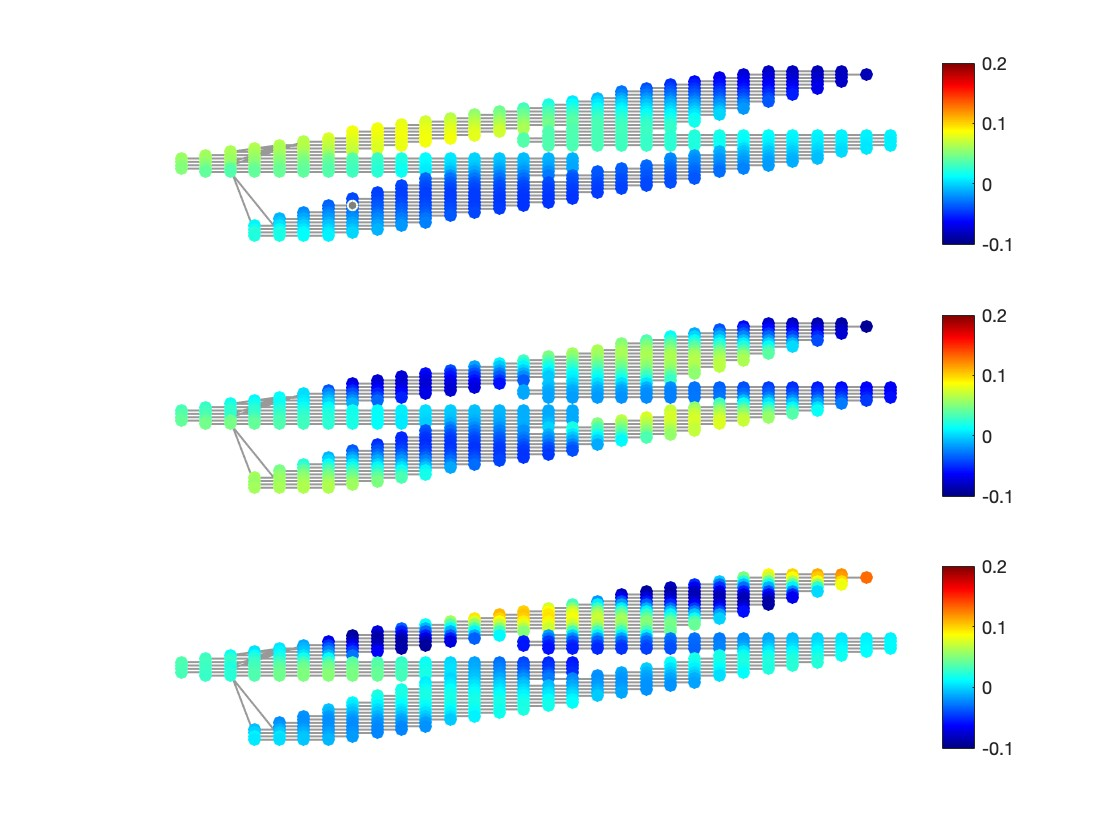
\includegraphics[width=12cm]{more_edges_second_ev.jpg}
	\caption{Spectral analysis of the graph for the 4th, 8th and 12th eigenvectors with more edges}
	\label{fig:MoreEdgesSpectralRepresentationSecondEv}
\end{figure}

\end{document}